\documentclass[a4paper,12pt]{report}
%\usepackage[a4paper,inner=1.7cm, outer=2.7cm, top=2cm, bottom=2cm, bindingoffset=1.2cm]{geometry} 
\usepackage[english]{babel} % use the english babel package. 
\usepackage[scaled=.92]{helvet} % tells you to use the helvetica font. 
\usepackage{multicol}

% Graphics Packages and Declarations
\usepackage{graphicx} % allows you to use pictures in your document.
\usepackage{caption} % allows you to have captions
\usepackage{subcaption} % allows you to use subcaptions and subgraphics.
\usepackage{wrapfig} % allows you to wrap text around your picture.
\DeclareGraphicsExtensions{.eps,.png,.pdf}


\usepackage{enumitem}% have your lists look nicer.
%\usepackage{fancyhdr} % allows you to have nice looking headers.
\usepackage{amsmath} % allows you to write math formula.
\usepackage{index} % allows you to use indexes that are automatically generated.
\usepackage{hyperref} % allows you to insert hyperlinks.
\usepackage{gensymb} % allows you to use symbols. 
% path information
\graphicspath{ 	{C:/Users/LocalAdmin/Desktop/LaTeX Master Thesis/MSView_tutorial} % MS view path
			{C:/Users/LocalAdmin/Desktop/LaTeX Master Thesis } % main path
		}



\begin{document}
\title{MS View tutorial}
\maketitle
\tableofcontents %Automatically generates a table of contents page.
\chapter{Morningstar View Tutorial}
\section{Viewing Charge Controller Data using MSView}

% adapted from the MS word document.
\paragraph{}
Here’s how to view live data using MSView from your PC:

\subsection{Step 1: Downloading the Program}
First, download MSView from Morningstar’s Corporate Website, located here:
\href{https://www.morningstarcorp.com/msview/}{https://www.morningstarcorp.com/msview/}
Figure \ref{fig:ms-website} shows what the website looks like.


\begin{figure}[h]
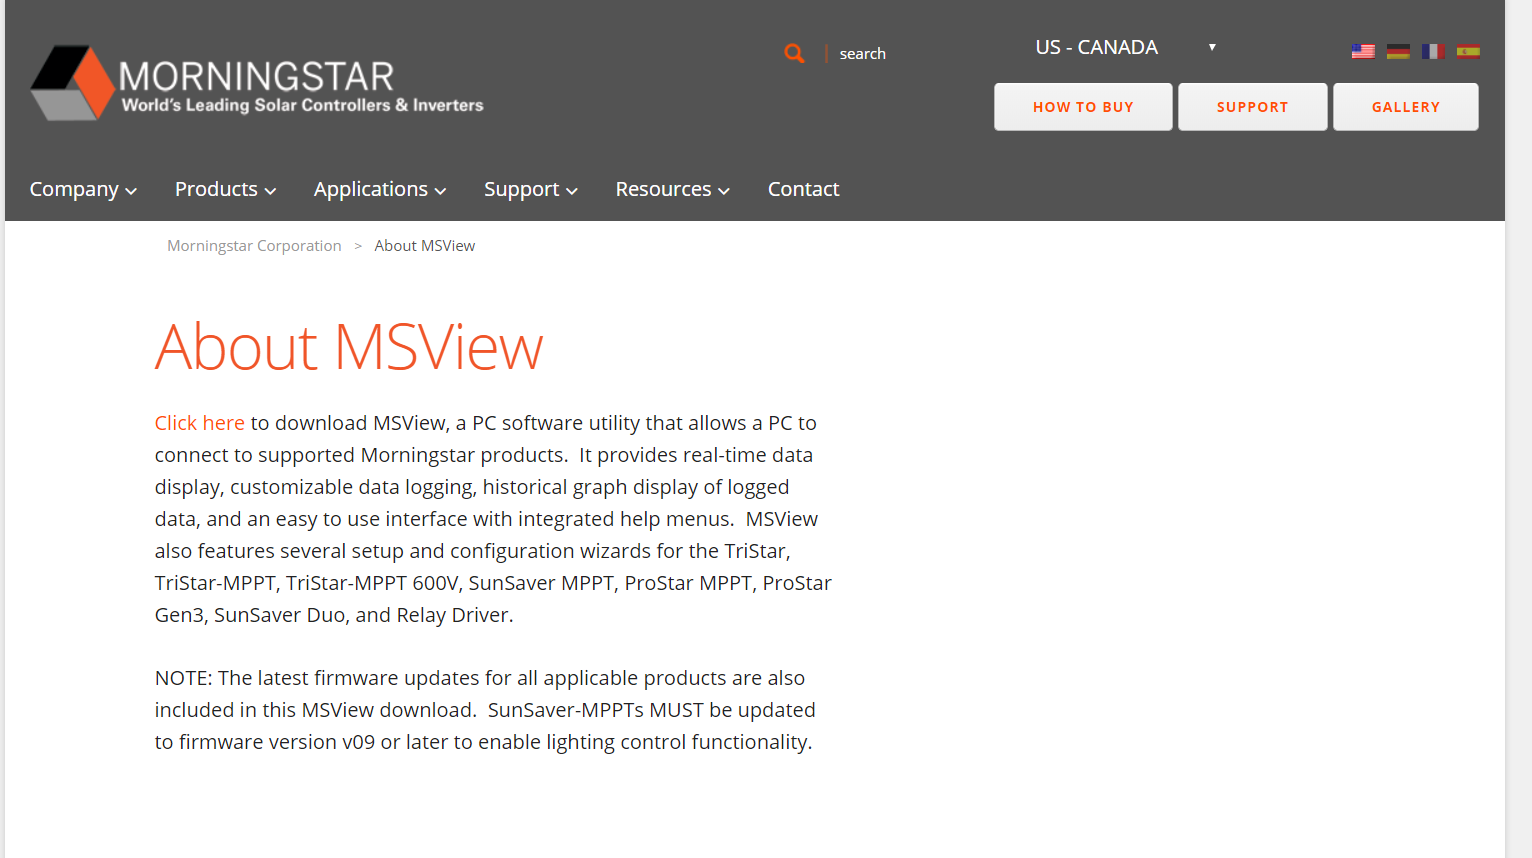
\includegraphics[width=\textwidth]{./graphics/tsmppt_troubleshooting/ms_1.png}
\caption{\label{fig:ms-website} Menu 1}
\end{figure}

\subsection{Step 2: Connecting the Morningstar}
If you’re using a RS-232 to USB serial connector to connect your PC, connect it now.

\subsection{Step 3: Powering the Morningstar}
Connect a 12V power supply to the battery terminal of the Tristar MPPT Charge Controller. It should draw approximately 189mA of current just for management.

\subsection{Step 4: Using MSView}
Open MSView.
Under Devices, select Search for Connected Devices. Your Tristar MPPT should show up under whatever virtual COM port you connected your RS-232 to USB connector to. Double-click it. You should see something like this appear.

\begin{figure}[h]
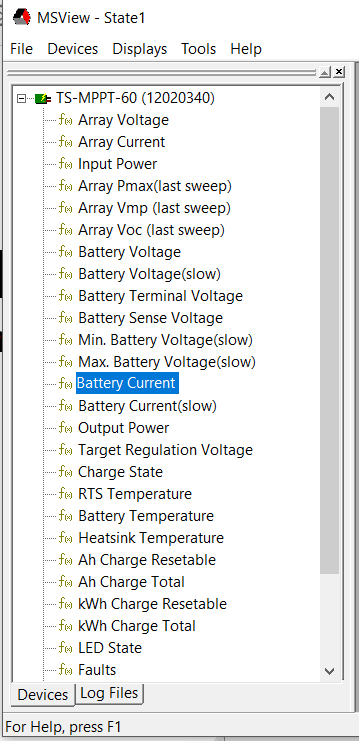
\includegraphics[width=0.7\columnwidth,angle=90,scale=0.75]{./graphics/tsmppt_troubleshooting/ms_2.png}
\caption{\label{fig:ms-website} First Menu upon initialization}
\end{figure}

\subsection{Step 5: Viewing Live Data}

Under Displays, select New. 
Select ‘State’ when a dialog box saying New Display appears and press OK.
Drag and drop whatever variables you want. Our Tristar MPPT can log:
\begin{itemize}
	\item Array Voltage (Array is shorthand for our solar panel array), 
	\item Array Current, Input Power (how much power our solar panels are producing), 
	\item Array Pmax, 
	\item Array Vmp, 
	\item Array Voc, 
	\item Battery Voltage (The Voltage of our Battery), 
	\item Battery Voltage (slow), 
	\item Battery Terminal Voltage, 
	\item Battery Sense Voltage (there’s a remote voltage sensor port on our Tristar MPPT that we can connect for safety), 
	\item Min. Battery Voltage (slow), 
	\item Max. Battery Voltage (slow), 
	\item Battery Current, 
	\item Battery Current(slow), 
	\item Output Power (how much power we’re consuming), 
	\item target regulation voltage, 
	\item charge state (Float, equalization, etc.), 
	\item RTS temperature, 
	\item Battery Temperature, 
	\item Heatsink Temperature, 
	\item Ah Charge Resetable, 
	\item Ah Charge Total, 
	\item kWh Charge Resetable, 
	\item kWh Charge Total, 
	\item LED State, Faults (did someone change the DIP switch?), 
	\item Faults Daily, 
	\item Alarms (did someone overcharge?), 
	\item Alarms Daily, 
	\item Hourmeter (how long have we been using this thing?),
	\item Settings Switches(the state of our DIP switch).
\end{itemize}

\subsection{Step 6: Programming the Tristar MPPT using MSView}

There are many different types of batteries: Lithium Ion, Lead-Acid, Lithium Polymer batteries, LiFePO4 batteries, etc. Each one of them requires its own different programming. The Tristar MPPT has 7 built-in programmable settings. To custom-program our Tristar MPPT to handle a battery, follow these steps:
\paragraph{}
Under Tools, click Tristar MPPT Setup Wizard. Read and click OK for both of the warnings against switching DIP switches while the power is applied.
\begin{figure}[!htb]
	\centering
	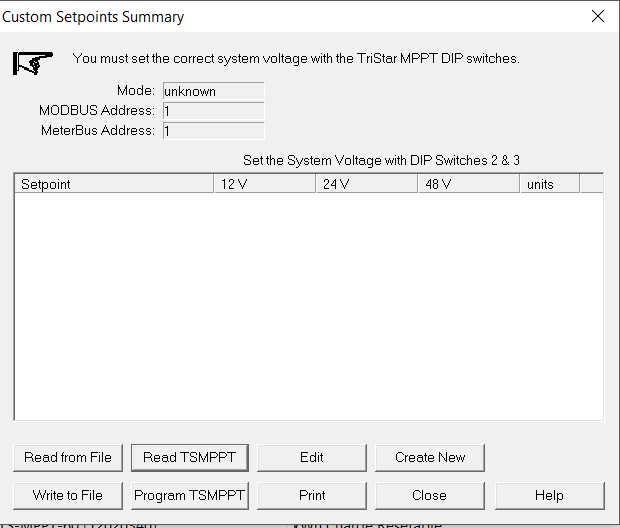
\includegraphics[width=0.6\columnwidth,scale=0.8]{./graphics/tsmppt_troubleshooting/ms_3.png}
	\caption{\label{fig:ts_setup_wizard} TSMPPT Setup Wizard}
\end{figure}

When on the screen that looks like Figure\ref{fig:ts_setup_wizard}, Click Read TSMPPT. Make sure it’s set to Solar Charge Control. If you’re using a serial connection, make sure you’re using the right COM port.
On our Tristar MPPT, the MODBUS address is 1.

% \begin{figure}%
	% \parbox{1.2in}{
		% 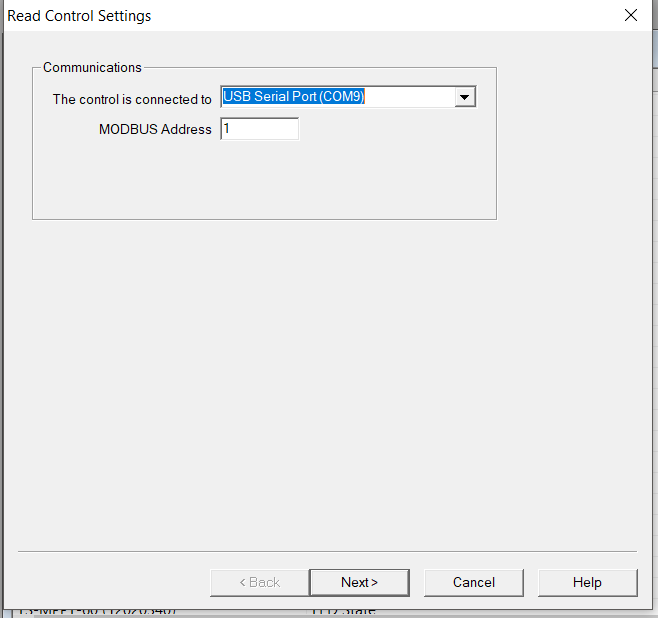
\includegraphics[width=0.6\columnwidth,scale=0.5]{./graphics/tsmppt_troubleshooting/ms_4.png}
		% \caption{First Figure}
	% }%
	% \qquad
	% \begin{minipage}{1.2in}%
		% 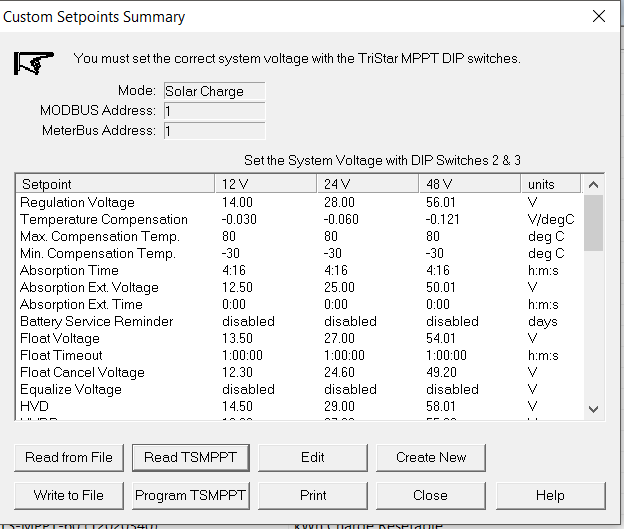
\includegraphics[width=\columnwidth,scale=0.7]{./graphics/tsmppt_troubleshooting/ms_5.png}
	% \end{minipage}%
	% \caption{Here are two figures side-by-side.}%
	% \label{fig:1figs}%
% \end{figure}

\begin{figure}[!htb]
	\centering
	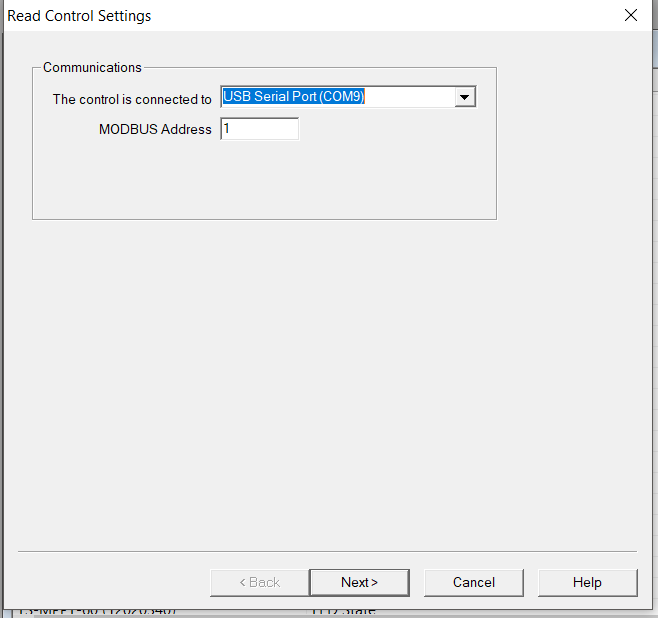
\includegraphics[width=\columnwidth]{./graphics/tsmppt_troubleshooting/ms_4.png}
	\caption{\label{fig:my-label} Communications settings}
\end{figure}

\begin{figure}[!htb]
	\centering
	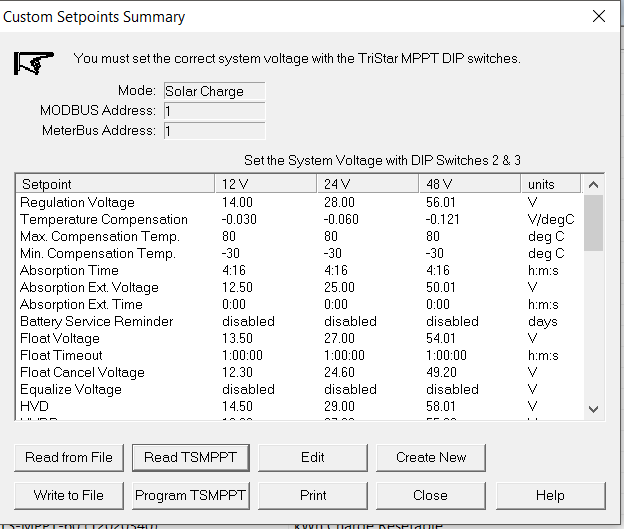
\includegraphics[width=\columnwidth]{./graphics/tsmppt_troubleshooting/ms_5.png}
	\caption{\label{fig:my-label} Tristar Morningstar Charge Settings Screen}
\end{figure}

The Setup wizard should look something like this afterwards if reading the settings was successful.

Read the settings you extracted from the Tristar MPPT first before you reprogram it. If the settings are not to your liking (i.e. the batteries will not charge properly), you can reprogram the Tristar MPPT. If you have a file already saved, click Read from File, and all your previously made changes will be loaded. 
If you don’t have a file made already, then click Edit. This will allow you to make your own custom settings.
You can change all these settings shown below:
  
 
\begin{figure}[!htb]
	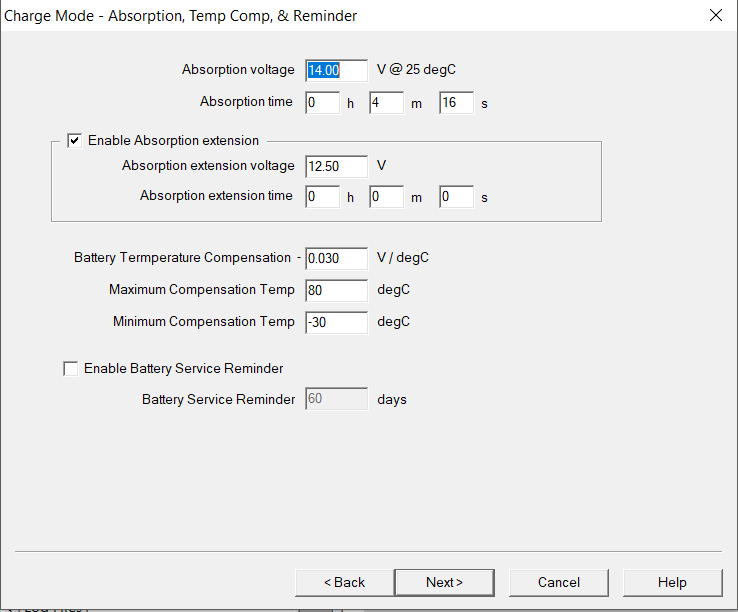
\includegraphics[width=\columnwidth,height=\textwidth,scale=0.5]{./graphics/tsmppt_troubleshooting/ms_6.png}
	\caption{\label{fig:settings-1} Absorption, Temperature Compensation, and Reminder Settings}
\end{figure}

\begin{figure}[!htb]
	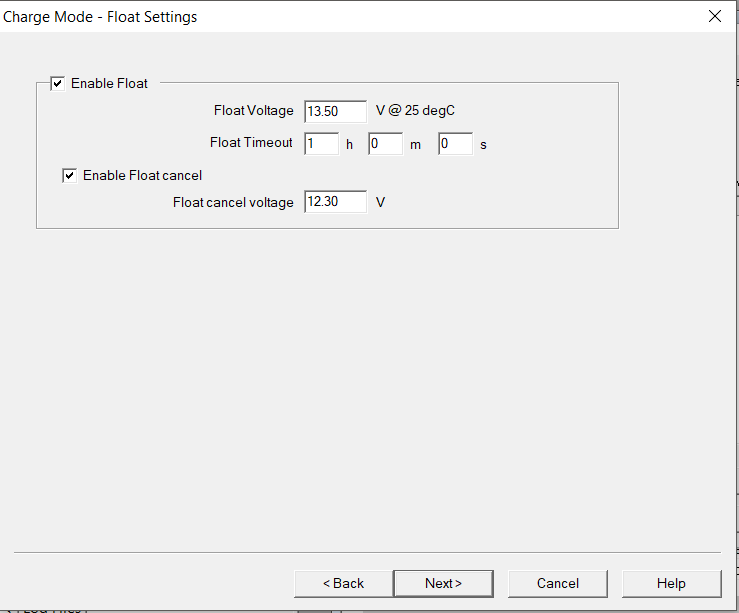
\includegraphics[width=\textwidth,height=\textwidth,scale=0.5]{./graphics/tsmppt_troubleshooting/ms_7.png}
	\caption{\label{fig:settings-2} Float Settings}
	
\end{figure}
\begin{figure}[!htb]
	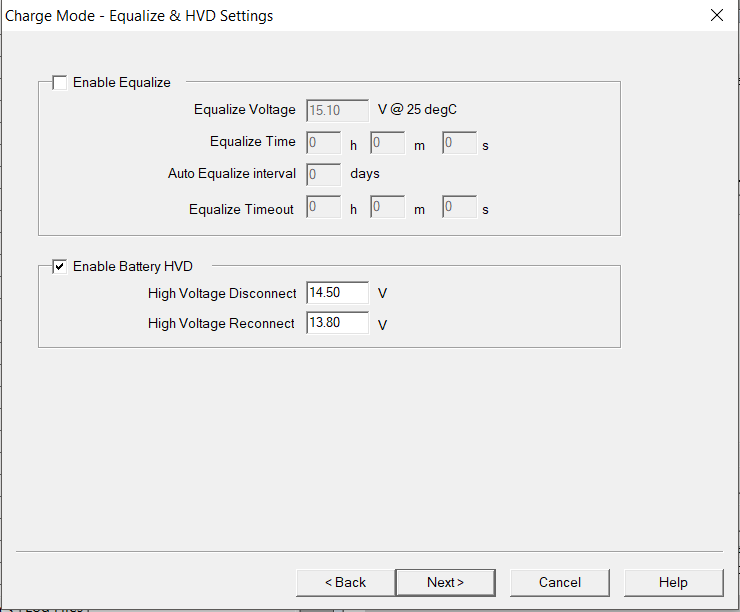
\includegraphics[width=\textwidth,height=\textwidth]{./graphics/tsmppt_troubleshooting/ms_8.png}
	\caption{\label{fig:settings-3} Equalize and HVD Settings}
\end{figure}
\begin{figure}[!htb]
	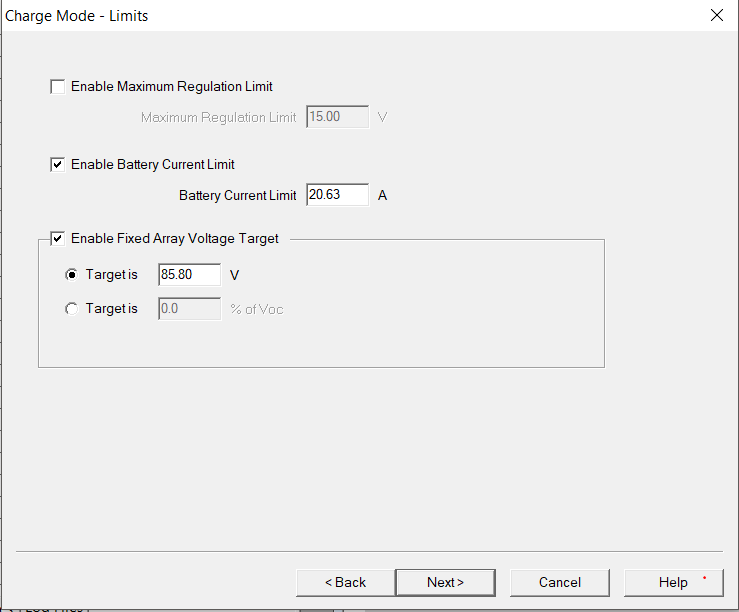
\includegraphics[width=\textwidth,height=\textwidth]{./graphics/tsmppt_troubleshooting/ms_9.png}
	\caption{\label{fig:settings-4} Limits Settings}
\end{figure}
\begin{figure}[!htb]
	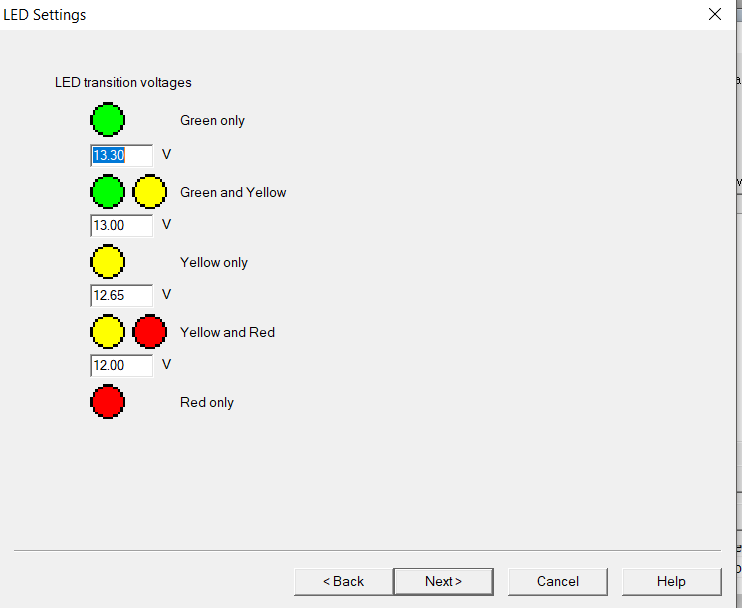
\includegraphics[width=\textwidth,height=\textwidth]{./graphics/tsmppt_troubleshooting/ms_10.png}
	\caption{\label{fig:settings-5} LED Settings}
\end{figure}
\begin{figure}[!htb]
	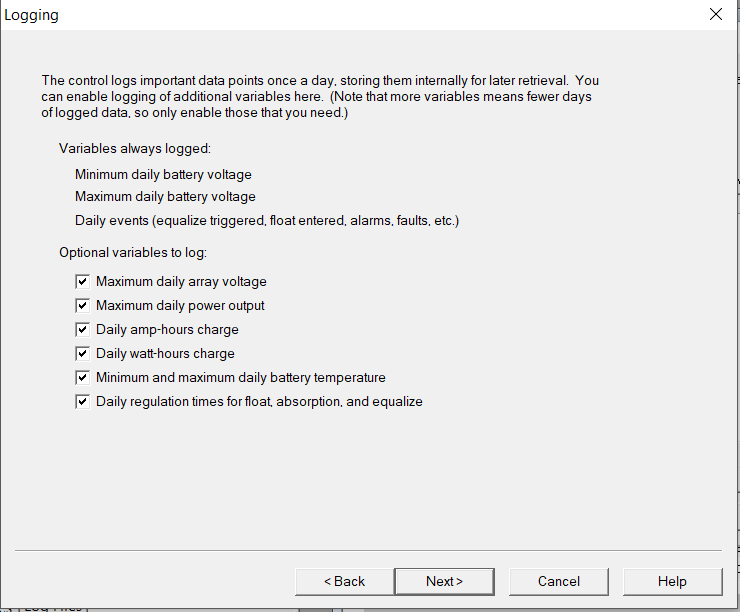
\includegraphics[width=\textwidth,height=\textwidth]{./graphics/tsmppt_troubleshooting/ms_11.png}
	\caption{\label{fig:settings-6} Logger Settings}
\end{figure}
\begin{figure}[!htb]
	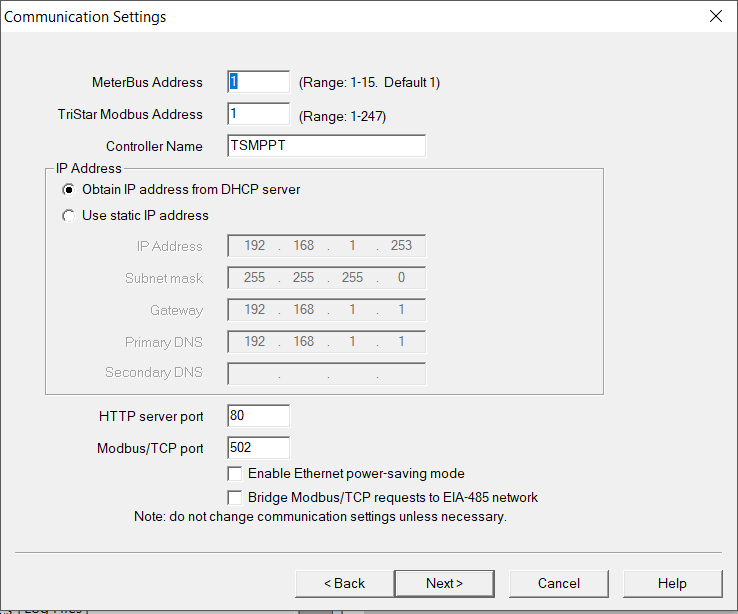
\includegraphics[width=\textwidth,height=\textwidth]{./graphics/tsmppt_troubleshooting/ms_12.png}
	\caption{\label{fig:settings-7} Commmunication Settings}
\end{figure}
\begin{figure}[!htb]
	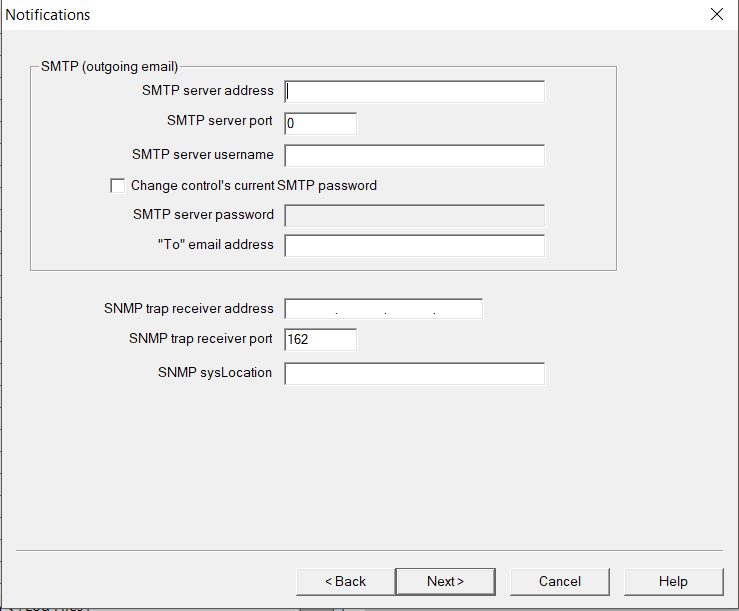
\includegraphics[width=\textwidth,height=\textwidth]{./graphics/tsmppt_troubleshooting/ms_13.png}
	\caption{\label{fig:settings-8} Mail Server Settings (TCP Exclusive)}
\end{figure}
\begin{figure}[!htb]
	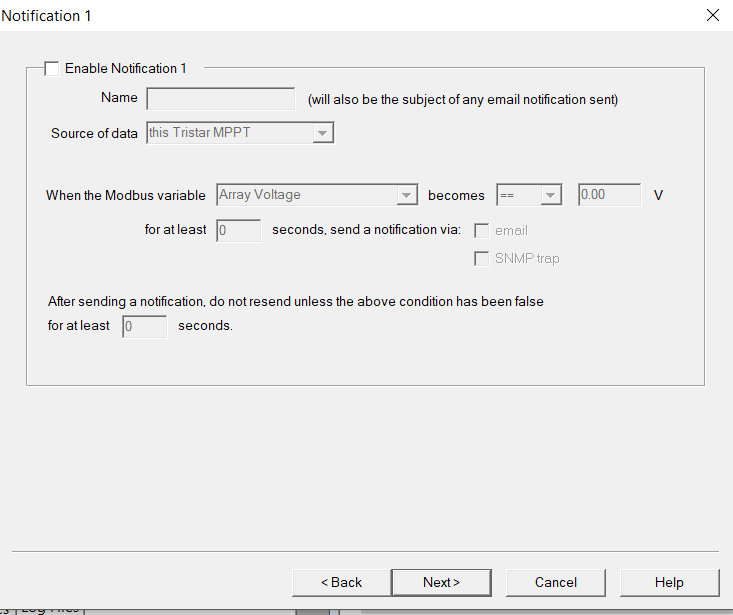
\includegraphics[width=\textwidth,height=\textwidth]{./graphics/tsmppt_troubleshooting/ms_14.png}
	\caption{\label{fig:settings-9} Notification 1}
\end{figure}
\begin{figure}[!htb]
	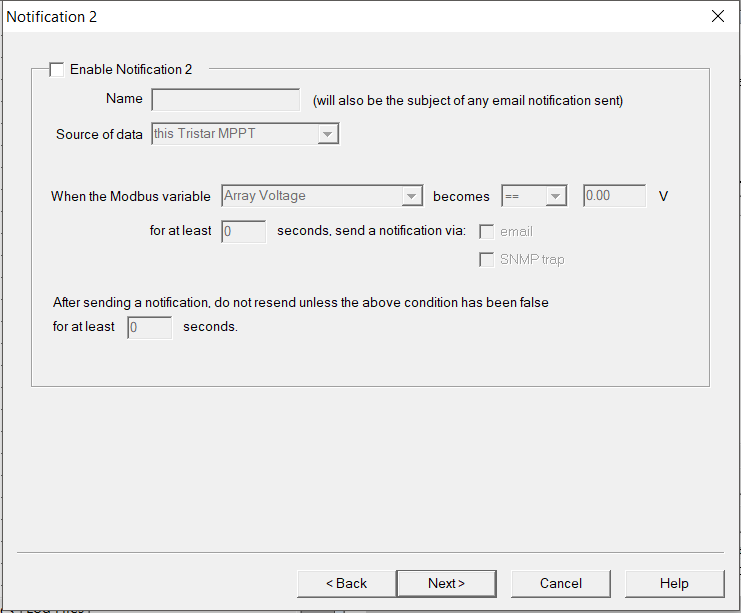
\includegraphics[width=\textwidth,height=\textwidth]{./graphics/tsmppt_troubleshooting/ms_15.png}
	\caption{\label{fig:settings-10} Notification 2}
\end{figure}
\begin{figure}[!htb]
	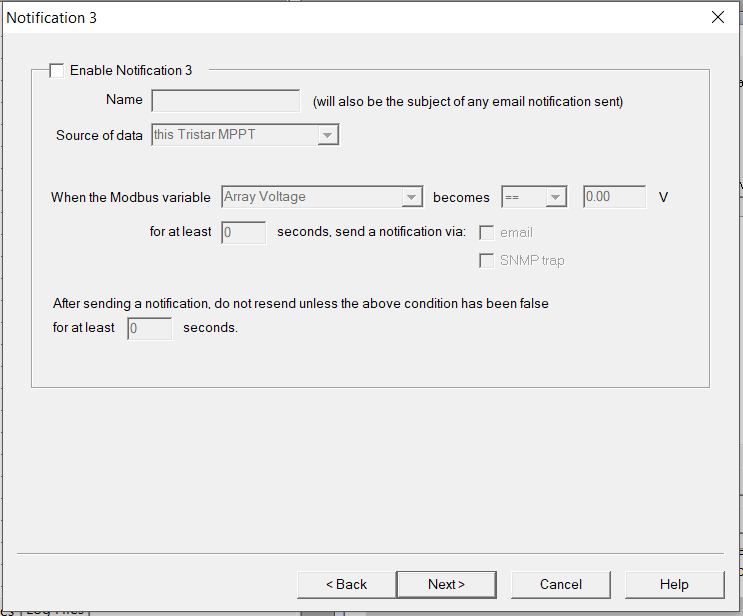
\includegraphics[width=\textwidth,height=\textwidth]{./graphics/tsmppt_troubleshooting/ms_16.png}
	\caption{\label{fig:settings-11} Notification 3}
\end{figure}
\begin{figure}[!htb]
	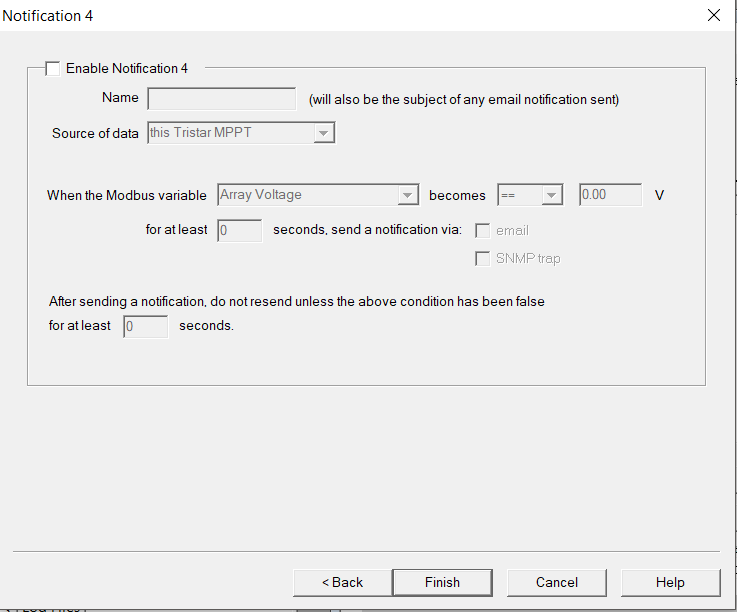
\includegraphics[width=\textwidth,height=\textwidth]{./graphics/tsmppt_troubleshooting/ms_17.png}
	\caption{\label{fig:settings-12} Notification 4}
\end{figure}
\begin{figure}[!htb]
	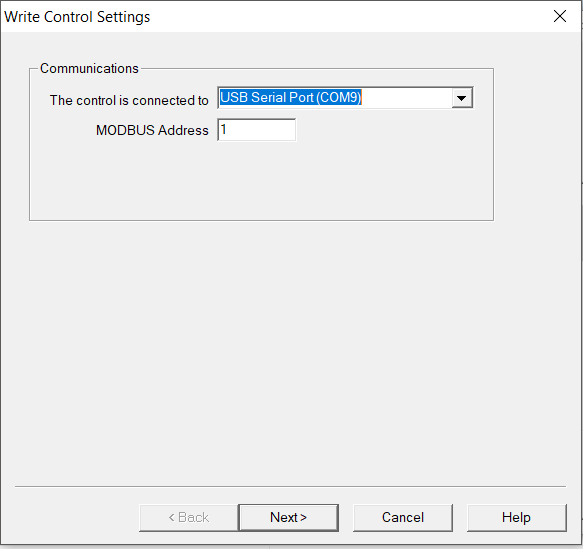
\includegraphics[width=\textwidth,height=\textwidth]{./graphics/tsmppt_troubleshooting/ms_18.png}
	\caption{\label{fig:settings-13} Write Control Communication Settings}
\end{figure}
\begin{figure}[!htb]
	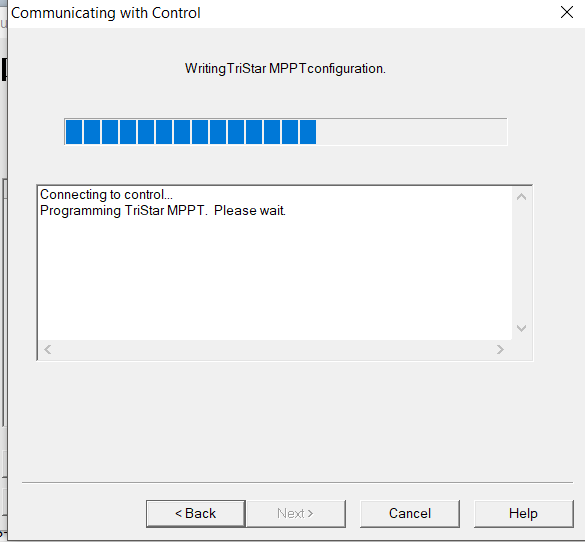
\includegraphics[width=\textwidth,height=\textwidth]{./graphics/tsmppt_troubleshooting/ms_19.png}
	\caption{\label{fig:settings-14} Writing Settings to the Tristar Screen}
\end{figure}

\paragraph{}
Once all of your changes are made, you can save it to a file, just in case you need to reprogram the Tristar MPPT. Save it by using Write to File.

Once you have your settings loaded, you need to program the Tristar MPPT. Click Program TSMPPT, and make sure the COM port is correct.

Now, your Tristar should be ready to be used with your batteries!

\subsection{Final Step}
Oh, one more thing! If you want to use custom charging settings, DIP switches 4,5, and 6 must be switched on! That’s how the custom settings work! It even says so in MSView! \\
Also, this is a CHARGE CONTROLLER! It won’t manage all your batteries for you! You must use a BMS system for that. Luckily, we have one. I’ve got a separate document for that. It can help you balance out the charges on your batteries so that every battery has an even charge, and none of them use too many life cycles at the same time.
 \\


% makes an index.


%metadata
% page numbering data
\pagenumbering{roman} %sets page numbering style to "roman numerals"
\setcounter{page}{2} % start page numbering on page 2.
\end{document}